\documentclass{scrartcl}

\usepackage{amssymb}
\usepackage{amsmath}
\usepackage{cancel}		%for strikethroughs
\usepackage{tikz}
\usetikzlibrary{calc,intersections,through,backgrounds,patterns}
\usetikzlibrary{decorations.text, decorations.markings, arrows, arrows.meta}

\tikzset{->-/.style={decoration={
			markings,
			mark=at position #1 with {\arrow{>}}},postaction={decorate}}}

\def\centerarc[#1](#2)(#3:#4:#5)% Syntax: [draw options] (center) (initial angle:final angle:radius)
{ \draw[#1] ($(#2)+({#5*cos(#3)},{#5*sin(#3)})$) arc (#3:#4:#5); }

%TO DO: define custom arrowhead (open triangle 30?)

\begin{document}
	
	%\begin{figure}
	%	\centering
	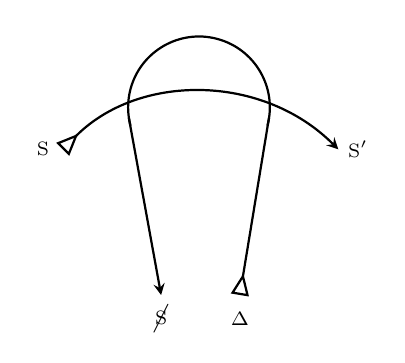
\begin{tikzpicture}
	
	\node at (-0.5,1.85) {{\scriptsize S}};
	\node at (3.5,1.85) {{\scriptsize S$^\prime$}};
	\node at (1,-0.25) {{\scriptsize \cancel{S}}};
	\node at (2,-0.3) {{\scriptsize $\Delta$}};
	
	\draw [open triangle 45 reversed-stealth, thick]	(-0.25,1.85) to[bend left=45] (3.25,1.85);
	
	\draw [->,>=stealth, thick]	(0.59,2.25)--(1,0);
	\draw [-open triangle 45 reversed, thick]	(2.37,2.25)--(2,0);
	
	\draw[thick] (2.35,2.15) arc (-15:195:9mm);
	
	%to[bend left=120]
	%then I tried: to[out=247.5,in=270]
	
	\end{tikzpicture}
	%	\caption{Graph of Desire 1}
	%\end{figure}
	
	\vspace{0.75cm}
		
	%\begin{figure}
	%	\centering
	\hspace{-0.2cm}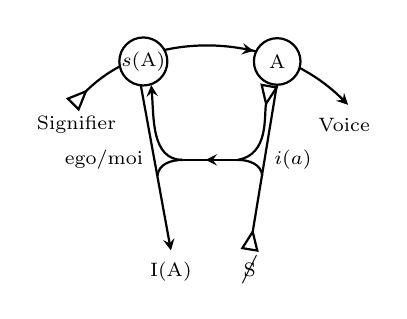
\begin{tikzpicture}
	
	%labels
	\node at (-0.2,1.6) {{\scriptsize Signifier}};
	\node at (3.2,1.6) {{\scriptsize Voice}};
	\node at (1,-0.27) {{\scriptsize I(A)}};		%
	\node at (2,-0.2) {{\scriptsize \cancel{S}}};	%NB: these last two aren't level
	\node at (0.15,1.15) {{\scriptsize ego/moi}};
	\node at (2.55,1.15) {{\scriptsize $i(a)$}};
	
	%upper arrow
	\draw [open triangle 45 reversed-stealth, thick]	(-0.25,1.85) to[bend left=45] (3.25,1.85);
	\draw [->,>=stealth,thick]	(2,2.535) to[bend right=-10] (2.05,2.535);	%upper-mid arrowhead (right)
	
	%lower arrows
	\draw [->,>=stealth, thick]	(0.59,2.25)--(1,0);
	\draw [-open triangle 45 reversed, thick]	(2.37,2.25)--(2,0);
	%\draw[thick] (2.35,2.15) arc (-15:195:9mm);
	\centerarc[->,>=stealth,thick](1.48,2.28)(27:153:0.97)	%top arc, changed to an arrow
	%easier solution: use the old arc, add an arrowhead
	
	%circles
	\node[circle,thick,draw=black,fill=white,inner sep=0pt,minimum size=4pt] (Sa) at (0.65,2.4) {{\scriptsize $s$(A)}};
	\node[circle,thick,draw=black,fill=white,inner sep=0pt,minimum size=4pt] (A) at (2.35,2.4) {\textcolor{white}{{\scriptsize s(A)}}};
	\node at (2.35,2.4) {{\scriptsize A}};
	%this is a cheap hack to get the size of the circles right -- fix later
	
	%middle arrows
	\draw [->-=.585, >=stealth, thick] (1.85,1.15)--(1.15,1.15);
	\draw [->,>=stealth,thick] (1.15,1.15) to[out=180,in=275] (0.75,2.1);
	\draw [-open triangle 45 reversed,thick] (1.85,1.15) to[out=10,in=260] (2.25,2.1);
	%\node at (0.835,0.95) {\textcolor{red}{.}};
	\draw [thick] (1.15,1.15) to[out=180,in=85] (0.83,0.95);
	%\node at (2.16,0.95) {\textcolor{red}{.}};
	\draw [thick] (1.85,1.15) to[out=0,in=95] (2.16,0.95);
	
	\end{tikzpicture}
	%	\caption{Graph of Desire 2}
	%\end{figure}
	
	\vspace{0.75cm}
	
	%\begin{figure}
	%	\centering
	\hspace{0.35cm}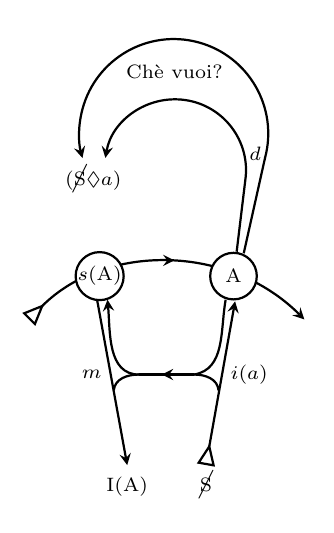
\begin{tikzpicture}
	
	%labels
	%\node at (-0.2,1.6) {{\scriptsize Signifier}};		%omitted from these ones
	%\node at (3.2,1.6) {{\scriptsize Voice}};
	\node at (1,-0.27) {{\scriptsize I(A)}};
	\node at (2,-0.2) {{\scriptsize \cancel{S}}};	%NB: these last two aren't level
	\node at (0.55,1.15) {{\scriptsize $m$}};
	\node at (2.55,1.15) {{\scriptsize $i(a)$}};
	
	%upper arrow
	\draw [open triangle 45 reversed-stealth, thick]	(-0.25,1.85) to[bend left=45] (3.25,1.85);
	\draw [->,>=stealth,thick]	(1.55,2.6)--(1.6,2.6);	%upper-mid arrowhead (center)
	
	%lower arrows
	\draw [->,>=stealth, thick]	(0.59,2.25)--(1,0);
	\draw [stealth-open triangle 45 reversed, thick]	(2.37,2.08)--(2,0);
	%\draw[thick] (2.35,2.15) arc (-15:195:9mm);
	\centerarc[->,>=stealth,thick](1.48,2.28)(27:153:0.97)	%top arc, changed to an arrow
	%easier solution: use the old arc, add an arrowhead
	
	%circles
	\node[circle,thick,draw=black,fill=white,inner sep=0pt,minimum size=4pt] (Sa) at (0.65,2.4) {{\scriptsize $s$(A)}};
	\node[circle,thick,draw=black,fill=white,inner sep=0pt,minimum size=4pt] (A) at (2.35,2.4) {\textcolor{white}{{\scriptsize s(A)}}};
	\node at (2.35,2.4) {{\scriptsize A}};
	%this is a cheap hack to get the size of the circles right -- fix later
	
	%middle arrows
	\draw [->-=.585, >=stealth, thick] (1.85,1.15)--(1.15,1.15);
	\draw [->,>=stealth,thick] (1.15,1.15) to[out=180,in=275] (0.75,2.1);
	\draw [thick] (1.85,1.15) to[out=10,in=260] (2.25,2.1);		%NB: different from graph 2
	%\node at (0.835,0.95) {\textcolor{red}{.}};
	\draw [thick] (1.15,1.15) to[out=180,in=85] (0.83,0.95);
	%\node at (2.16,0.95) {\textcolor{red}{.}};
	\draw [thick] (1.85,1.15) to[out=0,in=95] (2.16,0.95);
	
	%top labels
	\node at (0.57,3.65) {{\scriptsize (\cancel{S}$\,\!\lozenge a$)}};
	\node at (2.625,3.95) {{\scriptsize $d$}};
	
	%top part
	\draw[->,>=stealth,thick] (2.75,3.9) arc (-15:195:1.2cm);
	%\draw[->,>=stealth,thick] (2.5,4.2) arc (10:170:9mm);
	\draw[->,>=stealth,thick] (2.5,3.62) arc (-8:170:9mm);
	\draw [thick] (2.39,2.71)--(2.5,3.62);
	\draw [thick] (2.48,2.69)--(2.75,3.9);
	\node at (1.6,5) {{\scriptsize Ch\`{e} vuoi?}};
	
	\end{tikzpicture}
	%	\caption{Ch\`{e} vuoi?}
	%\end{figure}
	
	
	\vspace{0.75cm}
	
	
	%\begin{figure}
	%	\centering
	\hspace{-0.2cm}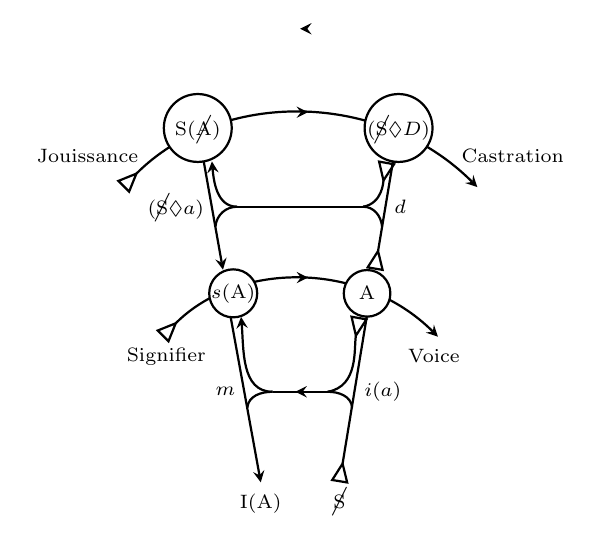
\begin{tikzpicture}
	
	%labels
	\node at (-0.2,1.6) {{\scriptsize Signifier}};
	\node at (3.2,1.6) {{\scriptsize Voice}};
	\node at (1,-0.27) {{\scriptsize I(A)}};		%
	\node at (2,-0.2) {{\scriptsize \cancel{S}}};	%NB: these last two aren't level
	\node at (0.55,1.15) {{\scriptsize $m$}};
	\node at (2.55,1.15) {{\scriptsize $i(a)$}};
	
	%lower horizontal arrow
	\draw [open triangle 45 reversed-stealth, thick]	(-0.25,1.85) to[bend left=45] (3.25,1.85);
	\draw [->,>=stealth,thick]	(1.55,2.6)--(1.6,2.6);	%upper-mid arrowhead (center)
	
	%lower arrows
	\draw [->,>=stealth, thick]	(0.59,2.25)--(1,0);
	\draw [-open triangle 45 reversed, thick]	(2.37,2.25)--(2,0);
	%\draw[thick] (2.35,2.15) arc (-15:195:9mm);
	\centerarc[open triangle 45 reversed-stealth, thick](1.48,2.28)(27:153:0.97)	%top arc, changed to an arrow
	%easier solution: use the old arc, add an arrowhead
	%but then here, I can't have two arrowheads unless I add both manually
	
	%bottom circles
	\node[circle,thick,draw=black,fill=white,inner sep=0pt,minimum size=4pt] (Sa) at (0.65,2.4) {{\scriptsize $s$(A)}};
	\node[circle,thick,draw=black,fill=white,inner sep=0pt,minimum size=4pt] (A) at (2.35,2.4) {\textcolor{white}{{\scriptsize s(A)}}};
	\node at (2.35,2.4) {{\scriptsize A}};
	%this is a cheap hack to get the size of the circles right -- fix later
	
	%middle arrows
	\draw [->-=.585, >=stealth, thick] (1.85,1.15)--(1.15,1.15);
	\draw [->,>=stealth,thick] (1.15,1.15) to[out=180,in=275] (0.75,2.1);
	\draw [-open triangle 45 reversed,thick] (1.85,1.15) to[out=10,in=260] (2.25,2.1);
	%\node at (0.835,0.95) {\textcolor{red}{.}};
	\draw [thick] (1.15,1.15) to[out=180,in=85] (0.83,0.95);
	%\node at (2.16,0.95) {\textcolor{red}{.}};
	\draw [thick] (1.85,1.15) to[out=0,in=95] (2.16,0.95);
	
	%top side arrows
		%\draw [thick,red] (0.68,1.75)--(0.2,4.5);		%check continuity with bottom line
	\draw [->,>=stealth,thick] (0.2,4.5)--(0.52,2.7);
		%\draw [thick,red] (2.29,1.75)--(2.75,4.5);		%check continuity with bottom line
	\draw [-open triangle 45 reversed,thick] (2.75,4.5)--(2.45,2.7);
	
	%top horizontal arrow
	\draw [open triangle 45 reversed-stealth, thick]	(-0.75,3.75) to[bend left=45] (3.75,3.75);
	\draw [->,>=stealth,thick]	(1.55,4.7)--(1.6,4.7);	%arrowhead (center)
	
	%top circles
	\node[circle,thick,draw=black,fill=white,inner sep=0pt,minimum size=4pt] (SD) at (0.2,4.5) {\textcolor{white}{{\scriptsize (\cancel{S}$\,\!\lozenge D$)}}};
	\node at (0.2,4.5) {{\scriptsize S(\cancel{A})}};
	\node[circle,thick,draw=black,fill=white,inner sep=0pt,minimum size=4pt] (SA) at (2.75,4.5) {{\scriptsize (\cancel{S}$\,\!\lozenge D$)}};
	%this is a cheap hack to get the size of the circles right -- fix later
	
	%top-mid arrows
	\draw [thick] (0.7,3.5)--(2.3,3.5);
		%\node at (0.38,4.075) {\textcolor{red}{.}};
		%\node at (2.6,4.07) {\textcolor{red}{.}};
	\draw [->,>=stealth,thick] (0.7,3.5) to[out=180,in=275] (0.38,4.075);
	\draw [-open triangle 45 reversed,thick] (2.3,3.5) to[out=10,in=260] (2.6,4.07);
		%\node at (0.43,3.25) {\textcolor{red}{.}};
	\draw [thick] (0.7,3.5) to[out=180,in=85] (0.425,3.25);
		%\node at (2.55,3.25) {\textcolor{red}{.}};
	\draw [thick] (2.3,3.5) to[out=0,in=95] (2.54,3.25);
	%
	%\node at (0.2,4.95) {\textcolor{red}{.}};
	%\node at (2.75,4.95) {\textcolor{red}{.}};
	\centerarc[open triangle 45 reversed-stealth, thick](1.48,4.3)(27:153:1.45)
	\draw [->,>=stealth,thick]	(1.55,5.76)--(1.5,5.76);
	
	%top labels
	\node at (-0.08,3.5) {{\scriptsize (\cancel{S}$\,\!\lozenge a$)}};
	\node at (2.77,3.5) {{\scriptsize $d$}};
	\node at (-1.2,4.15) {{\scriptsize Jouissance}};
	\node at (4.2,4.15) {{\scriptsize Castration}};
	
	\end{tikzpicture}
	%	\caption{Graph of Desire 3}
	%\end{figure}
	
	
\end{document}